% Created by tikzDevice version 0.12.3.1 on 2021-03-25 18:09:52
% !TEX encoding = UTF-8 Unicode
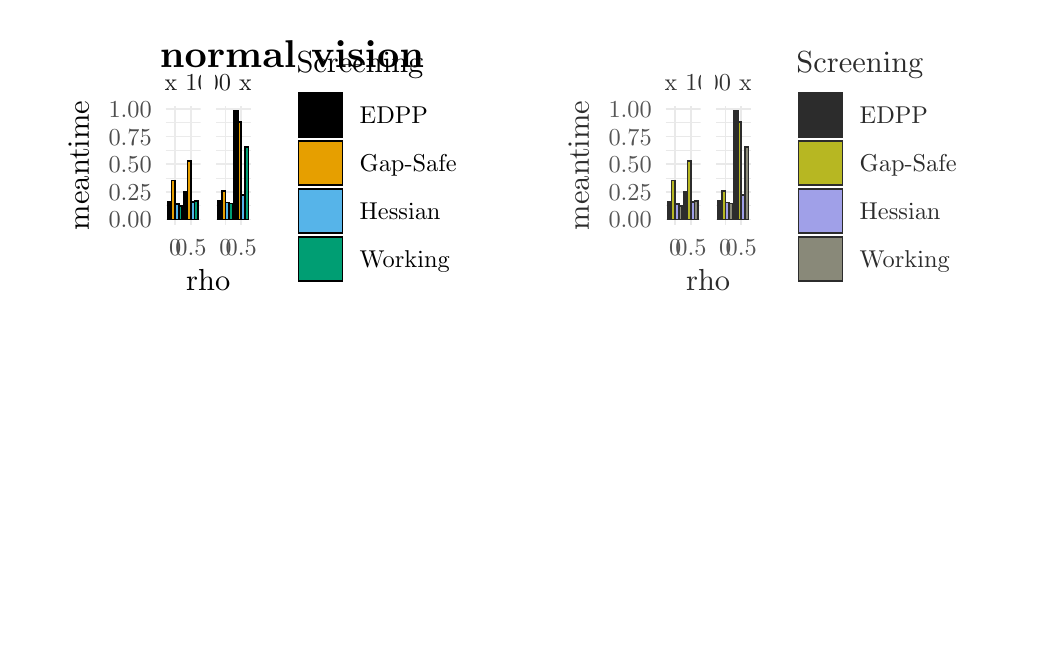
\begin{tikzpicture}[x=1pt,y=1pt]
\definecolor{fillColor}{RGB}{255,255,255}
\path[use as bounding box,fill=fillColor,fill opacity=0.00] (0,0) rectangle (361.35,216.81);
\begin{scope}
\path[clip] ( 49.82,145.50) rectangle ( 62.48,188.62);
\definecolor{drawColor}{gray}{0.92}

\path[draw=drawColor,line width= 0.3pt,line join=round] ( 49.82,152.46) --
	( 62.48,152.46);

\path[draw=drawColor,line width= 0.3pt,line join=round] ( 49.82,162.45) --
	( 62.48,162.45);

\path[draw=drawColor,line width= 0.3pt,line join=round] ( 49.82,172.44) --
	( 62.48,172.44);

\path[draw=drawColor,line width= 0.3pt,line join=round] ( 49.82,182.43) --
	( 62.48,182.43);

\path[draw=drawColor,line width= 0.6pt,line join=round] ( 49.82,147.46) --
	( 62.48,147.46);

\path[draw=drawColor,line width= 0.6pt,line join=round] ( 49.82,157.45) --
	( 62.48,157.45);

\path[draw=drawColor,line width= 0.6pt,line join=round] ( 49.82,167.44) --
	( 62.48,167.44);

\path[draw=drawColor,line width= 0.6pt,line join=round] ( 49.82,177.43) --
	( 62.48,177.43);

\path[draw=drawColor,line width= 0.6pt,line join=round] ( 49.82,187.42) --
	( 62.48,187.42);

\path[draw=drawColor,line width= 0.6pt,line join=round] ( 53.27,145.50) --
	( 53.27,188.62);

\path[draw=drawColor,line width= 0.6pt,line join=round] ( 59.02,145.50) --
	( 59.02,188.62);
\definecolor{drawColor}{RGB}{0,0,0}
\definecolor{fillColor}{RGB}{0,0,0}

\path[draw=drawColor,line width= 0.6pt,line cap=rect,fill=fillColor] ( 50.68,147.46) rectangle ( 51.98,153.73);
\definecolor{fillColor}{RGB}{230,159,0}

\path[draw=drawColor,line width= 0.6pt,line cap=rect,fill=fillColor] ( 51.98,147.46) rectangle ( 53.27,161.62);
\definecolor{fillColor}{RGB}{86,180,233}

\path[draw=drawColor,line width= 0.6pt,line cap=rect,fill=fillColor] ( 53.27,147.46) rectangle ( 54.57,152.98);
\definecolor{fillColor}{RGB}{0,158,115}

\path[draw=drawColor,line width= 0.6pt,line cap=rect,fill=fillColor] ( 54.57,147.46) rectangle ( 55.86,152.30);
\definecolor{fillColor}{RGB}{0,0,0}

\path[draw=drawColor,line width= 0.6pt,line cap=rect,fill=fillColor] ( 56.44,147.46) rectangle ( 57.73,157.34);
\definecolor{fillColor}{RGB}{230,159,0}

\path[draw=drawColor,line width= 0.6pt,line cap=rect,fill=fillColor] ( 57.73,147.46) rectangle ( 59.02,168.64);
\definecolor{fillColor}{RGB}{86,180,233}

\path[draw=drawColor,line width= 0.6pt,line cap=rect,fill=fillColor] ( 59.02,147.46) rectangle ( 60.32,153.70);
\definecolor{fillColor}{RGB}{0,158,115}

\path[draw=drawColor,line width= 0.6pt,line cap=rect,fill=fillColor] ( 60.32,147.46) rectangle ( 61.61,154.29);
\end{scope}
\begin{scope}
\path[clip] ( 67.98,145.50) rectangle ( 80.64,188.62);
\definecolor{drawColor}{gray}{0.92}

\path[draw=drawColor,line width= 0.3pt,line join=round] ( 67.98,152.46) --
	( 80.64,152.46);

\path[draw=drawColor,line width= 0.3pt,line join=round] ( 67.98,162.45) --
	( 80.64,162.45);

\path[draw=drawColor,line width= 0.3pt,line join=round] ( 67.98,172.44) --
	( 80.64,172.44);

\path[draw=drawColor,line width= 0.3pt,line join=round] ( 67.98,182.43) --
	( 80.64,182.43);

\path[draw=drawColor,line width= 0.6pt,line join=round] ( 67.98,147.46) --
	( 80.64,147.46);

\path[draw=drawColor,line width= 0.6pt,line join=round] ( 67.98,157.45) --
	( 80.64,157.45);

\path[draw=drawColor,line width= 0.6pt,line join=round] ( 67.98,167.44) --
	( 80.64,167.44);

\path[draw=drawColor,line width= 0.6pt,line join=round] ( 67.98,177.43) --
	( 80.64,177.43);

\path[draw=drawColor,line width= 0.6pt,line join=round] ( 67.98,187.42) --
	( 80.64,187.42);

\path[draw=drawColor,line width= 0.6pt,line join=round] ( 71.43,145.50) --
	( 71.43,188.62);

\path[draw=drawColor,line width= 0.6pt,line join=round] ( 77.18,145.50) --
	( 77.18,188.62);
\definecolor{drawColor}{RGB}{0,0,0}
\definecolor{fillColor}{RGB}{0,0,0}

\path[draw=drawColor,line width= 0.6pt,line cap=rect,fill=fillColor] ( 68.84,147.46) rectangle ( 70.13,154.10);
\definecolor{fillColor}{RGB}{230,159,0}

\path[draw=drawColor,line width= 0.6pt,line cap=rect,fill=fillColor] ( 70.13,147.46) rectangle ( 71.43,157.79);
\definecolor{fillColor}{RGB}{86,180,233}

\path[draw=drawColor,line width= 0.6pt,line cap=rect,fill=fillColor] ( 71.43,147.46) rectangle ( 72.72,153.68);
\definecolor{fillColor}{RGB}{0,158,115}

\path[draw=drawColor,line width= 0.6pt,line cap=rect,fill=fillColor] ( 72.72,147.46) rectangle ( 74.02,153.22);
\definecolor{fillColor}{RGB}{0,0,0}

\path[draw=drawColor,line width= 0.6pt,line cap=rect,fill=fillColor] ( 74.59,147.46) rectangle ( 75.89,186.66);
\definecolor{fillColor}{RGB}{230,159,0}

\path[draw=drawColor,line width= 0.6pt,line cap=rect,fill=fillColor] ( 75.89,147.46) rectangle ( 77.18,182.81);
\definecolor{fillColor}{RGB}{86,180,233}

\path[draw=drawColor,line width= 0.6pt,line cap=rect,fill=fillColor] ( 77.18,147.46) rectangle ( 78.48,156.30);
\definecolor{fillColor}{RGB}{0,158,115}

\path[draw=drawColor,line width= 0.6pt,line cap=rect,fill=fillColor] ( 78.48,147.46) rectangle ( 79.77,173.60);
\end{scope}
\begin{scope}
\path[clip] ( 49.82,188.62) rectangle ( 62.48,205.89);
\definecolor{drawColor}{gray}{0.10}

\node[text=drawColor,anchor=base,inner sep=0pt, outer sep=0pt, scale=  0.88] at ( 56.15,194.22) {100 x 10000};
\end{scope}
\begin{scope}
\path[clip] ( 67.98,188.62) rectangle ( 80.64,205.89);
\definecolor{drawColor}{gray}{0.10}

\node[text=drawColor,anchor=base,inner sep=0pt, outer sep=0pt, scale=  0.88] at ( 74.31,194.22) {10000 x 100};
\end{scope}
\begin{scope}
\path[clip] (  0.00,  0.00) rectangle (361.35,216.81);
\definecolor{drawColor}{gray}{0.30}

\node[text=drawColor,anchor=base,inner sep=0pt, outer sep=0pt, scale=  0.88] at ( 53.27,134.49) {0};

\node[text=drawColor,anchor=base,inner sep=0pt, outer sep=0pt, scale=  0.88] at ( 59.02,134.49) {0.5};
\end{scope}
\begin{scope}
\path[clip] (  0.00,  0.00) rectangle (361.35,216.81);
\definecolor{drawColor}{gray}{0.30}

\node[text=drawColor,anchor=base,inner sep=0pt, outer sep=0pt, scale=  0.88] at ( 71.43,134.49) {0};

\node[text=drawColor,anchor=base,inner sep=0pt, outer sep=0pt, scale=  0.88] at ( 77.18,134.49) {0.5};
\end{scope}
\begin{scope}
\path[clip] (  0.00,  0.00) rectangle (361.35,216.81);
\definecolor{drawColor}{gray}{0.30}

\node[text=drawColor,anchor=base east,inner sep=0pt, outer sep=0pt, scale=  0.88] at ( 44.87,144.43) {0.00};

\node[text=drawColor,anchor=base east,inner sep=0pt, outer sep=0pt, scale=  0.88] at ( 44.87,154.42) {0.25};

\node[text=drawColor,anchor=base east,inner sep=0pt, outer sep=0pt, scale=  0.88] at ( 44.87,164.41) {0.50};

\node[text=drawColor,anchor=base east,inner sep=0pt, outer sep=0pt, scale=  0.88] at ( 44.87,174.40) {0.75};

\node[text=drawColor,anchor=base east,inner sep=0pt, outer sep=0pt, scale=  0.88] at ( 44.87,184.39) {1.00};
\end{scope}
\begin{scope}
\path[clip] (  0.00,  0.00) rectangle (361.35,216.81);
\definecolor{drawColor}{RGB}{0,0,0}

\node[text=drawColor,anchor=base,inner sep=0pt, outer sep=0pt, scale=  1.10] at ( 65.23,121.75) {rho};
\end{scope}
\begin{scope}
\path[clip] (  0.00,  0.00) rectangle (361.35,216.81);
\definecolor{drawColor}{RGB}{0,0,0}

\node[text=drawColor,rotate= 90.00,anchor=base,inner sep=0pt, outer sep=0pt, scale=  1.10] at ( 22.11,167.06) {meantime};
\end{scope}
\begin{scope}
\path[clip] (  0.00,  0.00) rectangle (361.35,216.81);
\definecolor{drawColor}{RGB}{0,0,0}

\node[text=drawColor,anchor=base west,inner sep=0pt, outer sep=0pt, scale=  1.10] at ( 97.14,200.71) {Screening};
\end{scope}
\begin{scope}
\path[clip] (  0.00,  0.00) rectangle (361.35,216.81);
\definecolor{drawColor}{RGB}{0,0,0}
\definecolor{fillColor}{RGB}{0,0,0}

\path[draw=drawColor,line width= 0.6pt,line cap=rect,fill=fillColor] ( 97.85,177.19) rectangle (113.77,193.11);
\end{scope}
\begin{scope}
\path[clip] (  0.00,  0.00) rectangle (361.35,216.81);
\definecolor{drawColor}{RGB}{0,0,0}
\definecolor{fillColor}{RGB}{230,159,0}

\path[draw=drawColor,line width= 0.6pt,line cap=rect,fill=fillColor] ( 97.85,159.84) rectangle (113.77,175.77);
\end{scope}
\begin{scope}
\path[clip] (  0.00,  0.00) rectangle (361.35,216.81);
\definecolor{drawColor}{RGB}{0,0,0}
\definecolor{fillColor}{RGB}{86,180,233}

\path[draw=drawColor,line width= 0.6pt,line cap=rect,fill=fillColor] ( 97.85,142.50) rectangle (113.77,158.42);
\end{scope}
\begin{scope}
\path[clip] (  0.00,  0.00) rectangle (361.35,216.81);
\definecolor{drawColor}{RGB}{0,0,0}
\definecolor{fillColor}{RGB}{0,158,115}

\path[draw=drawColor,line width= 0.6pt,line cap=rect,fill=fillColor] ( 97.85,125.15) rectangle (113.77,141.08);
\end{scope}
\begin{scope}
\path[clip] (  0.00,  0.00) rectangle (361.35,216.81);
\definecolor{drawColor}{RGB}{0,0,0}

\node[text=drawColor,anchor=base west,inner sep=0pt, outer sep=0pt, scale=  0.88] at (119.98,182.12) {EDPP};
\end{scope}
\begin{scope}
\path[clip] (  0.00,  0.00) rectangle (361.35,216.81);
\definecolor{drawColor}{RGB}{0,0,0}

\node[text=drawColor,anchor=base west,inner sep=0pt, outer sep=0pt, scale=  0.88] at (119.98,164.77) {Gap-Safe};
\end{scope}
\begin{scope}
\path[clip] (  0.00,  0.00) rectangle (361.35,216.81);
\definecolor{drawColor}{RGB}{0,0,0}

\node[text=drawColor,anchor=base west,inner sep=0pt, outer sep=0pt, scale=  0.88] at (119.98,147.43) {Hessian};
\end{scope}
\begin{scope}
\path[clip] (  0.00,  0.00) rectangle (361.35,216.81);
\definecolor{drawColor}{RGB}{0,0,0}

\node[text=drawColor,anchor=base west,inner sep=0pt, outer sep=0pt, scale=  0.88] at (119.98,130.08) {Working};
\end{scope}
\begin{scope}
\path[clip] (  0.00,  0.00) rectangle (361.35,216.81);
\definecolor{drawColor}{RGB}{0,0,0}

\node[text=drawColor,anchor=base west,inner sep=0pt, outer sep=0pt, scale=  1.40] at ( 47.73,202.32) {\bfseries normal vision};
\end{scope}
\begin{scope}
\path[clip] (230.49,145.50) rectangle (243.15,188.62);
\definecolor{drawColor}{RGB}{233,233,233}

\path[draw=drawColor,line width= 0.3pt,line join=round] (230.49,152.46) --
	(243.15,152.46);

\path[draw=drawColor,line width= 0.3pt,line join=round] (230.49,162.45) --
	(243.15,162.45);

\path[draw=drawColor,line width= 0.3pt,line join=round] (230.49,172.44) --
	(243.15,172.44);

\path[draw=drawColor,line width= 0.3pt,line join=round] (230.49,182.43) --
	(243.15,182.43);

\path[draw=drawColor,line width= 0.6pt,line join=round] (230.49,147.46) --
	(243.15,147.46);

\path[draw=drawColor,line width= 0.6pt,line join=round] (230.49,157.45) --
	(243.15,157.45);

\path[draw=drawColor,line width= 0.6pt,line join=round] (230.49,167.44) --
	(243.15,167.44);

\path[draw=drawColor,line width= 0.6pt,line join=round] (230.49,177.43) --
	(243.15,177.43);

\path[draw=drawColor,line width= 0.6pt,line join=round] (230.49,187.42) --
	(243.15,187.42);

\path[draw=drawColor,line width= 0.6pt,line join=round] (233.95,145.50) --
	(233.95,188.62);

\path[draw=drawColor,line width= 0.6pt,line join=round] (239.70,145.50) --
	(239.70,188.62);
\definecolor{drawColor}{RGB}{44,44,44}
\definecolor{fillColor}{RGB}{44,44,44}

\path[draw=drawColor,line width= 0.6pt,line cap=rect,fill=fillColor] (231.36,147.46) rectangle (232.65,153.73);
\definecolor{fillColor}{RGB}{183,183,34}

\path[draw=drawColor,line width= 0.6pt,line cap=rect,fill=fillColor] (232.65,147.46) rectangle (233.95,161.62);
\definecolor{fillColor}{RGB}{160,160,232}

\path[draw=drawColor,line width= 0.6pt,line cap=rect,fill=fillColor] (233.95,147.46) rectangle (235.24,152.98);
\definecolor{fillColor}{RGB}{137,137,121}

\path[draw=drawColor,line width= 0.6pt,line cap=rect,fill=fillColor] (235.24,147.46) rectangle (236.54,152.30);
\definecolor{fillColor}{RGB}{44,44,44}

\path[draw=drawColor,line width= 0.6pt,line cap=rect,fill=fillColor] (237.11,147.46) rectangle (238.41,157.34);
\definecolor{fillColor}{RGB}{183,183,34}

\path[draw=drawColor,line width= 0.6pt,line cap=rect,fill=fillColor] (238.41,147.46) rectangle (239.70,168.64);
\definecolor{fillColor}{RGB}{160,160,232}

\path[draw=drawColor,line width= 0.6pt,line cap=rect,fill=fillColor] (239.70,147.46) rectangle (240.99,153.70);
\definecolor{fillColor}{RGB}{137,137,121}

\path[draw=drawColor,line width= 0.6pt,line cap=rect,fill=fillColor] (240.99,147.46) rectangle (242.29,154.29);
\end{scope}
\begin{scope}
\path[clip] (248.65,145.50) rectangle (261.31,188.62);
\definecolor{drawColor}{RGB}{233,233,233}

\path[draw=drawColor,line width= 0.3pt,line join=round] (248.65,152.46) --
	(261.31,152.46);

\path[draw=drawColor,line width= 0.3pt,line join=round] (248.65,162.45) --
	(261.31,162.45);

\path[draw=drawColor,line width= 0.3pt,line join=round] (248.65,172.44) --
	(261.31,172.44);

\path[draw=drawColor,line width= 0.3pt,line join=round] (248.65,182.43) --
	(261.31,182.43);

\path[draw=drawColor,line width= 0.6pt,line join=round] (248.65,147.46) --
	(261.31,147.46);

\path[draw=drawColor,line width= 0.6pt,line join=round] (248.65,157.45) --
	(261.31,157.45);

\path[draw=drawColor,line width= 0.6pt,line join=round] (248.65,167.44) --
	(261.31,167.44);

\path[draw=drawColor,line width= 0.6pt,line join=round] (248.65,177.43) --
	(261.31,177.43);

\path[draw=drawColor,line width= 0.6pt,line join=round] (248.65,187.42) --
	(261.31,187.42);

\path[draw=drawColor,line width= 0.6pt,line join=round] (252.10,145.50) --
	(252.10,188.62);

\path[draw=drawColor,line width= 0.6pt,line join=round] (257.86,145.50) --
	(257.86,188.62);
\definecolor{drawColor}{RGB}{44,44,44}
\definecolor{fillColor}{RGB}{44,44,44}

\path[draw=drawColor,line width= 0.6pt,line cap=rect,fill=fillColor] (249.52,147.46) rectangle (250.81,154.10);
\definecolor{fillColor}{RGB}{183,183,34}

\path[draw=drawColor,line width= 0.6pt,line cap=rect,fill=fillColor] (250.81,147.46) rectangle (252.10,157.79);
\definecolor{fillColor}{RGB}{160,160,232}

\path[draw=drawColor,line width= 0.6pt,line cap=rect,fill=fillColor] (252.10,147.46) rectangle (253.40,153.68);
\definecolor{fillColor}{RGB}{137,137,121}

\path[draw=drawColor,line width= 0.6pt,line cap=rect,fill=fillColor] (253.40,147.46) rectangle (254.69,153.22);
\definecolor{fillColor}{RGB}{44,44,44}

\path[draw=drawColor,line width= 0.6pt,line cap=rect,fill=fillColor] (255.27,147.46) rectangle (256.56,186.66);
\definecolor{fillColor}{RGB}{183,183,34}

\path[draw=drawColor,line width= 0.6pt,line cap=rect,fill=fillColor] (256.56,147.46) rectangle (257.86,182.81);
\definecolor{fillColor}{RGB}{160,160,232}

\path[draw=drawColor,line width= 0.6pt,line cap=rect,fill=fillColor] (257.86,147.46) rectangle (259.15,156.30);
\definecolor{fillColor}{RGB}{137,137,121}

\path[draw=drawColor,line width= 0.6pt,line cap=rect,fill=fillColor] (259.15,147.46) rectangle (260.45,173.60);
\end{scope}
\begin{scope}
\path[clip] (230.49,188.62) rectangle (243.15,205.89);
\definecolor{drawColor}{RGB}{49,49,49}

\node[text=drawColor,anchor=base,inner sep=0pt, outer sep=0pt, scale=  0.88] at (236.82,194.22) {100 x 10000};
\end{scope}
\begin{scope}
\path[clip] (248.65,188.62) rectangle (261.31,205.89);
\definecolor{drawColor}{RGB}{49,49,49}

\node[text=drawColor,anchor=base,inner sep=0pt, outer sep=0pt, scale=  0.88] at (254.98,194.22) {10000 x 100};
\end{scope}
\begin{scope}
\path[clip] (  0.00,  0.00) rectangle (361.35,216.81);
\definecolor{drawColor}{RGB}{85,85,85}

\node[text=drawColor,anchor=base,inner sep=0pt, outer sep=0pt, scale=  0.88] at (233.95,134.49) {0};

\node[text=drawColor,anchor=base,inner sep=0pt, outer sep=0pt, scale=  0.88] at (239.70,134.49) {0.5};
\end{scope}
\begin{scope}
\path[clip] (  0.00,  0.00) rectangle (361.35,216.81);
\definecolor{drawColor}{RGB}{85,85,85}

\node[text=drawColor,anchor=base,inner sep=0pt, outer sep=0pt, scale=  0.88] at (252.10,134.49) {0};

\node[text=drawColor,anchor=base,inner sep=0pt, outer sep=0pt, scale=  0.88] at (257.86,134.49) {0.5};
\end{scope}
\begin{scope}
\path[clip] (  0.00,  0.00) rectangle (361.35,216.81);
\definecolor{drawColor}{RGB}{85,85,85}

\node[text=drawColor,anchor=base east,inner sep=0pt, outer sep=0pt, scale=  0.88] at (225.54,144.43) {0.00};

\node[text=drawColor,anchor=base east,inner sep=0pt, outer sep=0pt, scale=  0.88] at (225.54,154.42) {0.25};

\node[text=drawColor,anchor=base east,inner sep=0pt, outer sep=0pt, scale=  0.88] at (225.54,164.41) {0.50};

\node[text=drawColor,anchor=base east,inner sep=0pt, outer sep=0pt, scale=  0.88] at (225.54,174.40) {0.75};

\node[text=drawColor,anchor=base east,inner sep=0pt, outer sep=0pt, scale=  0.88] at (225.54,184.39) {1.00};
\end{scope}
\begin{scope}
\path[clip] (  0.00,  0.00) rectangle (361.35,216.81);
\definecolor{drawColor}{RGB}{44,44,44}

\node[text=drawColor,anchor=base,inner sep=0pt, outer sep=0pt, scale=  1.10] at (245.90,121.75) {rho};
\end{scope}
\begin{scope}
\path[clip] (  0.00,  0.00) rectangle (361.35,216.81);
\definecolor{drawColor}{RGB}{44,44,44}

\node[text=drawColor,rotate= 90.00,anchor=base,inner sep=0pt, outer sep=0pt, scale=  1.10] at (202.78,167.06) {meantime};
\end{scope}
\begin{scope}
\path[clip] (  0.00,  0.00) rectangle (361.35,216.81);
\definecolor{drawColor}{RGB}{44,44,44}

\node[text=drawColor,anchor=base west,inner sep=0pt, outer sep=0pt, scale=  1.10] at (277.81,200.71) {Screening};
\end{scope}
\begin{scope}
\path[clip] (  0.00,  0.00) rectangle (361.35,216.81);
\definecolor{drawColor}{RGB}{44,44,44}
\definecolor{fillColor}{RGB}{44,44,44}

\path[draw=drawColor,line width= 0.6pt,line cap=rect,fill=fillColor] (278.52,177.19) rectangle (294.44,193.11);
\end{scope}
\begin{scope}
\path[clip] (  0.00,  0.00) rectangle (361.35,216.81);
\definecolor{drawColor}{RGB}{44,44,44}
\definecolor{fillColor}{RGB}{183,183,34}

\path[draw=drawColor,line width= 0.6pt,line cap=rect,fill=fillColor] (278.52,159.84) rectangle (294.44,175.77);
\end{scope}
\begin{scope}
\path[clip] (  0.00,  0.00) rectangle (361.35,216.81);
\definecolor{drawColor}{RGB}{44,44,44}
\definecolor{fillColor}{RGB}{160,160,232}

\path[draw=drawColor,line width= 0.6pt,line cap=rect,fill=fillColor] (278.52,142.50) rectangle (294.44,158.42);
\end{scope}
\begin{scope}
\path[clip] (  0.00,  0.00) rectangle (361.35,216.81);
\definecolor{drawColor}{RGB}{44,44,44}
\definecolor{fillColor}{RGB}{137,137,121}

\path[draw=drawColor,line width= 0.6pt,line cap=rect,fill=fillColor] (278.52,125.15) rectangle (294.44,141.08);
\end{scope}
\begin{scope}
\path[clip] (  0.00,  0.00) rectangle (361.35,216.81);
\definecolor{drawColor}{RGB}{44,44,44}

\node[text=drawColor,anchor=base west,inner sep=0pt, outer sep=0pt, scale=  0.88] at (300.66,182.12) {EDPP};
\end{scope}
\begin{scope}
\path[clip] (  0.00,  0.00) rectangle (361.35,216.81);
\definecolor{drawColor}{RGB}{44,44,44}

\node[text=drawColor,anchor=base west,inner sep=0pt, outer sep=0pt, scale=  0.88] at (300.66,164.77) {Gap-Safe};
\end{scope}
\begin{scope}
\path[clip] (  0.00,  0.00) rectangle (361.35,216.81);
\definecolor{drawColor}{RGB}{44,44,44}

\node[text=drawColor,anchor=base west,inner sep=0pt, outer sep=0pt, scale=  0.88] at (300.66,147.43) {Hessian};
\end{scope}
\begin{scope}
\path[clip] (  0.00,  0.00) rectangle (361.35,216.81);
\definecolor{drawColor}{RGB}{44,44,44}

\node[text=drawColor,anchor=base west,inner sep=0pt, outer sep=0pt, scale=  0.88] at (300.66,130.08) {Working};
\end{scope}
\end{tikzpicture}
